\chapter{Introduction}
\begchap{M}ath is more than numbers! In the United States (and perhaps other countries around the world), our school system imprints in us distinct memories of math, almost all of which involves finding the value of some variable $x$. Yet, mathematicians do much more than solve for $x$; else mathematics would be quite a boring profession! Mathematics is the language behind our universe and the mechanism with which we describe interactions.  While school also tends to establish in us the notion that calculus is the pinnacle of mathematics, there is much more to mathematics than solving integrals. What began as cavemen counting the number stones before them had since developed into a very rich language which encompasses systems of logic and naturally describes the world around us. As such, we don't necessarily use the conventions of English grammar to find some unknown, we use language to convey ideas. Mathematics is very similar, in that we are more interested in ideas rather than variables and unknowns. 

Further, the question has been asked many times: what is mathematics research? Mathematicians spend their time finding and identifying patterns and proving new statements based on older statements and thus furthering our system of logic. For example, based on the fact that $a + b = 2$ and $a = b$, we can reasonably find that $a = b = 1$. In a similar fashion (though not necessarily algebraically), researchers identify relationships and attempt to find new conclusions based on existing principles (which may often result in the establishment of new principles for others to use, repeating the cycle). However, a key aspect here is how to ask the right question. We are not gifted by God a worksheet of math problems to solve to understand the universe, and thus, in mathematics, it is just as important to ask the right questions as it is to solve them. Given the two original statements about $a$, and $b$, we were not asked to do anything. However, our brains usually subconsciously ask the question of what is $a$ and what is $b$, which leads us to find their specific values. 

Though again, we emphasize that mathematics is not about finding values. One of the most famous theorems in all of mathematics, the Hairy Ball theorem (yes, that is the official name), uses mathematics to prove that a hairy ball will always have some sort of cowlick and can never be combed flat. Nowhere did we mention, or the researchers solve, for some specific variable. Though in this book we will not cover the mechanisms to prove such a theorem (this would usually require mathematics on the level of Graduate courses), we will guide you through an introduction of the basic mechanisms of proof, just as an English book would introduce you to the rules of grammar. In the modern era, our skills of solving for variables are becoming increasingly redundant because of calculators and AI; and thus, the time is more ripe than ever to learn mathematical proofs and unlock the deeper logical reasoning that constitutes, formally, the field of mathematics. We use our systems of logic to further understand specific objects or phenomenon in mathematics or the real world; often contributing to the system of logic along the way. 

Though you don't have to be a math PhD to start learning math proofs. In fact, the most prestigious math competition for high schoolers in the US (USAMO) and in the world (IMO) are both proof-based competitions in which you are given 6 questions, and a total of 9 hours for your response in which you will need to prove your answer!

Now to the question of why I wrote this book. I find that proofs in math are usually only taught in introductory Analysis classes for students in the US, and across the globe, there has been a silent shift seemingly away from proof-based math and towards numerics. While it makes sense to build from the basics, delaying the introduction of proofs until college is often counterproductive. I find that even in top "math talent" pools, there is often a lack of understanding of proofs in math, even though mathematics is, at its core, about using logic and numbers to prove statements. 

Thus, I wrote this book in order to bridge that gap and help bring the understanding of math proofs earlier. I believe waiting until sophomore year of undergraduate schooling with Real Analysis is far too long a delay to introduce proof-based math, and can at times dissuade those from doing math who may otherwise excel in the "real world of math". While numerical calculations form the sprint, proof-based math is closer to a triathlon; the best sprinter does not always win. I hope this book brings exposure to what proof-based math is, bridges your knowledge of regular math to applications in proof settings, and invokes your curiosity for the beauty of proofs! 

In the following chapter, we will introduce a proof to bridge our common knowledge of solving for a variable into a mathematical proof. In subsequent chapters, we will learn the basic mechanisms of logic, sets, and techniques of proof. After which, we will dive deeper into advanced strategies, techniques, and methods, rounding off with lots of practice. 

\section{An Example to Begin}
In around 7th or 8th grade, we are taught in school the method to find the length given the following scenario: we have a ladder propped up against a wall. The base of the ladder is 6 feet away of the wall, and the top of the ladder touches the wall a height of 8 feet from the bottom. We may assume the ladder is straight, and we are asked to find the length (height?) of the ladder.

We set up this problem by first drawing it out:

\begin{center}
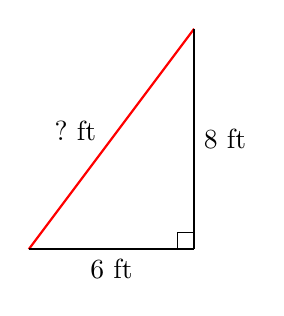
\begin{tikzpicture}[scale=0.35]
  % Ground and wall
  \draw[thick, black] (0,0) -- (6,0); % ground
  \draw[thick, black] (6,0) -- (6,8);        % wall

  % Triangle sides
  \draw[thick, red] (0,0) -- (6,8);         % ladder (hypotenuse)
  \draw[thick] (0,0) -- (6,0);         % base
  \draw[thick] (6,0) -- (6,8);         % height

  % Right angle box
  \draw (5.4,0) -- (5.4,.6) -- (6,.6);

  % Labels
  \node[below] at (3,0) {$6$ ft};
  \node[right] at (6,4) {$8$ ft};
  \node[left]  at (2.8,4.3) {$?$ ft};
\end{tikzpicture}
\end{center}

\begin{exercise}
    Try solving it for yourself before moving on!
\end{exercise}

Now, we need a tool from our toolbox of techniques to figure this out. That tool is the Pythagorean theorem. 
\begin{theorem} [Pythagorean Theorem]
Given a right triangle with legs of length $a$, $b$ and the hypotenuse length $c$, 
\begin{center}
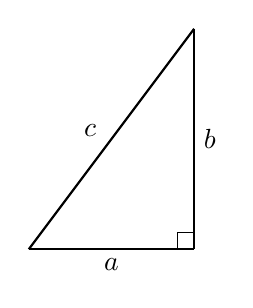
\begin{tikzpicture}[scale=0.35]
  % Ground and wall
  \draw[thick, black] (0,0) -- (6,0); % ground
  \draw[thick, black] (6,0) -- (6,8);        % wall

  % Triangle sides
  \draw[thick] (0,0) -- (6,8);         % ladder (hypotenuse)
  \draw[thick] (0,0) -- (6,0);         % base
  \draw[thick] (6,0) -- (6,8);         % height

  % Right angle box
  \draw (5.4,0) -- (5.4,.6) -- (6,.6);

  % Labels
  \node[below] at (3,0) {$a$};
  \node[right] at (6,4) {$b$};
  \node[left]  at (2.8,4.3) {$c$};
\end{tikzpicture}
\end{center}
The following holds true.
\[
a^2 + b^2 = c^2
\]
\end{theorem}

Using this theorem, we are now able to calculate the length of the ladder. 
\[6^2 + 8^2 = 100 \]
\[c^2 = 100 \]
\[ c = \pm 10\]

Since a length of $-10$ feet does not make sense in the real world, we choose $c = 10$. Thus, the length of the ladder is $10$ feet.

Now this was a painfully elaborate process of solving a quite simple problem. Most of us now would be able to do this process in our head and come to the conclusion that the answer is 10 feet. 

But what if we had to \emph{prove} our answer? We have used the Pythagorean Theorem as a fact of life, something our teacher told us and something we have since memorized. But where did it come from? \emph{Why} is it true? If we were to prove our answer, we would need to prove the Pythagorean theorem is true. This is the question a mathematician asks, and the same question Pythagoras asked 2600 years ago\footnote{Though there is now historical evidence that this relation was known across Babylon, Egypt, and India some 1000 years earlier; Pythagoras is credited with the first formal proof of this relation.}. And the answer is a \textbf{proof}.

The following is one of many, many beautiful proofs of the Pythagorean Theorem.
\begin{proof}
Consider the following diagram.
\begin{center}
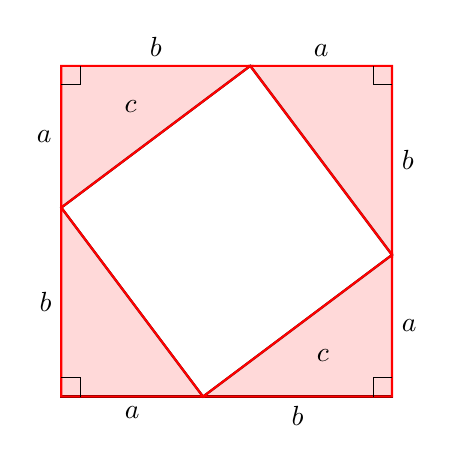
\begin{tikzpicture}[scale=0.6]

  % a=3, b=4, a+b=7
  % Inner square corners: (3,0), (7,3), (4,7), (0,4)

  % Four blue triangles
  \fill[red!15] (0,0) -- (3,0) -- (0,4) -- cycle;  % bottom-left
  \fill[red!15] (3,0) -- (7,0) -- (7,3) -- cycle;  % bottom-right
  \fill[red!15] (7,3) -- (7,7) -- (4,7) -- cycle;  % top-right
  \fill[red!15] (0,4) -- (0,7) -- (4,7) -- cycle;  % top-left

  % Inner tilted square
  \fill[white!15] (3,0) -- (7,3) -- (4,7) -- (0,4) -- cycle;

  % Outer square
  \draw[thick] (0,0) rectangle (7,7);

  % Inner tilted square outline
  \draw[thick] (3,0) -- (7,3) -- (4,7) -- (0,4) -- cycle;

  % Triangle outlines
  \draw[thick, red] (0,0) -- (3,0) -- (0,4) -- cycle;
  \draw[thick, red] (3,0) -- (7,0) -- (7,3) -- cycle;
  \draw[thick, red] (7,3) -- (7,7) -- (4,7) -- cycle;
  \draw[thick, red] (0,4) -- (0,7) -- (4,7) -- cycle;

  % Right angle boxes
  \draw (0.4,0) -- (0.4,0.4) -- (0,0.4);
  \draw (6.6,0) -- (6.6,0.4) -- (7,0.4);
  \draw (7,6.6) -- (6.6,6.6) -- (6.6,7);
  \draw (0.4,7) -- (0.4,6.6) -- (0,6.6);

  % Outer square side labels
  \node[below] at (1.5,0) {$a$};
  \node[below] at (5.0,0) {$b$};
  \node[right] at (7,1.5) {$a$};
  \node[right] at (7,5.0) {$b$};
  \node[above] at (5.5,7) {$a$};
  \node[above] at (2.0,7) {$b$};
  \node[left]  at (0,5.5) {$a$};
  \node[left]  at (0,2.0) {$b$};

  % Hypotenuse labels
  \node[below right] at (5.2,1.2) {$c$};
  \node[above left]  at (1.8,5.8) {$c$};
\end{tikzpicture}
\end{center}

The larger outer square has side length $a + b$. Therefore, its area is $(a + b)^2 = a^2 + 2ab + b^2$. We then try to count the area by finding the area of the triangles and the smaller inner square. We know the area of each smaller triangle is $\frac{1}{2}ab$, and the area of the central square is $c^2$. Thus, by this method of counting, we have the area is $4 \times \frac{1}{2}ab + c^2 = 2ab + c^2$.

Let $A$ be the area of the entire figure. Through our two methods of counting, we have that $A = a^2 + 2ab + b^2$, and through the second method, we have $A = 2ab + c^2$. Therefore, we have the following.
\[
a^2 + 2ab + b^2 = 2ab + c^2
\]

Which after simplifying gives us 
\begin{equation*}
    \boxed{a^2 + b^2 = c^2}
\end{equation*}
\end{proof}

This proof should immediately raise questions. Why does this work? How do we know the center quadrilateral is a square? How does this prove the Pythagorean Theorem for all triangles? If we were to prove this, how would we think of this method? 
\begin{exercise}
    Try to see if you can answer these yourself, before moving on. See how far you can get! 
\end{exercise}


Why does this work? This is perhaps an important point. We can prove the theorem this way because of our setup. Because in our setup we assumed the triangle was right-angled, with side $c$ being opposite the right angle, we are allowed to make any such construction. Then, since $a, b,$ and $c$ are all side lengths of the original triangle, we can use our constructed figure to make claims about the original triangle. But if we were to suspend the assumption that the triangle is right, or that $c$ is opposite the right angle, this proof would be very different, and we may not even be able to prove anything. The Pythagorean Theorem only works for right angled triangles with the specific setup demonstrated, so altering any of these properties moves us away from proving the Pythagorean Theorem.

How do we know the center quadrilateral is a square? This is a more mathematical question. We assumed in our proof that the center quadrilateral is a square, but astute readers will notice that we haven't actually proved this. Left unexplained, this is a hole in our proof, a hole in our logic, and the duty is upon us to patch the hole before our logic becomes invalidated!

Fortunately, the fix is easy. 
\begin{center}
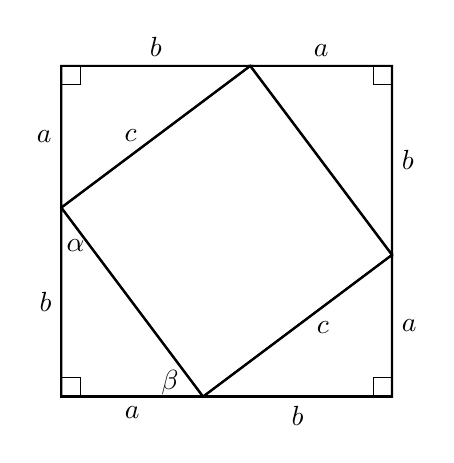
\begin{tikzpicture}[scale=0.6]

  % Outer square
  \draw[thick] (0,0) rectangle (7,7);

  % Inner tilted square
  \draw[thick] (3,0) -- (7,3) -- (4,7) -- (0,4) -- cycle;

  % Triangle outlines
  \draw[thick] (0,0) -- (3,0) -- (0,4) -- cycle;
  \draw[thick] (3,0) -- (7,0) -- (7,3) -- cycle;
  \draw[thick] (7,3) -- (7,7) -- (4,7) -- cycle;
  \draw[thick] (0,4) -- (0,7) -- (4,7) -- cycle;

  % Right angle boxes at OUTER corners
  \draw (0.4,0) -- (0.4,0.4) -- (0,0.4);
  \draw (6.6,0) -- (6.6,0.4) -- (7,0.4);
  \draw (7,6.6) -- (6.6,6.6) -- (6.6,7);
  \draw (0.4,7) -- (0.4,6.6) -- (0,6.6);

  % Outer square side labels
  \node[below] at (1.5,0) {$a$};
  \node[below] at (5.0,0) {$b$};
  \node[right] at (7,1.5) {$a$};
  \node[right] at (7,5.0) {$b$};
  \node[above] at (5.5,7) {$a$};
  \node[above] at (2.0,7) {$b$};
  \node[left]  at (0,5.5) {$a$};
  \node[left]  at (0,2.0) {$b$};

  % Hypotenuse labels
  \node[below right] at (5.2,1.8) {$c$};
  \node[above left]  at (1.8,5.2) {$c$};

  % Alpha (opposite a) and beta (opposite b)
  % labeled on bottom-left triangle only
  \node at (0.3,3.2) {$\alpha$};
  \node at (2.3,0.3) {$\beta$};

\end{tikzpicture}
\end{center}

First note that all the triangles are congruent to each other (they are the same triangle just copied and moved around and rearranged). This is because they have the same side lengths, and if you're still skeptical, they also have the same angle in between $b$ and $a$, which is always opposite the side $c$. If you're still not fully convinced, try making a mental picture and cutting out the triangles and stacking them on top of each other, they are truly copies of the same triangle\footnote{For those of you who may have taken a Geometry class in high school, you might recall that we can use Side-Angle-Side (SAS) or Side-Side-Side (SSS) congruence to prove this.}!

Next, notice that since all the triangles are congruent, we can then find out even more angles. We will just fill them in on the diagram. 

\begin{center}
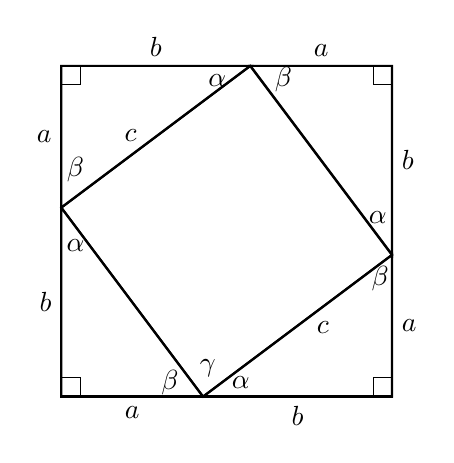
\begin{tikzpicture}[scale=0.6]
  % Outer square
  \draw[thick] (0,0) rectangle (7,7);
  % Inner tilted square
  \draw[thick] (3,0) -- (7,3) -- (4,7) -- (0,4) -- cycle;
  % Triangle outlines
  \draw[thick] (0,0) -- (3,0) -- (0,4) -- cycle;
  \draw[thick] (3,0) -- (7,0) -- (7,3) -- cycle;
  \draw[thick] (7,3) -- (7,7) -- (4,7) -- cycle;
  \draw[thick] (0,4) -- (0,7) -- (4,7) -- cycle;
  % Right angle boxes at OUTER corners
  \draw (0.4,0) -- (0.4,0.4) -- (0,0.4);
  \draw (6.6,0) -- (6.6,0.4) -- (7,0.4);
  \draw (7,6.6) -- (6.6,6.6) -- (6.6,7);
  \draw (0.4,7) -- (0.4,6.6) -- (0,6.6);
  % Outer square side labels
  \node[below] at (1.5,0) {$a$};
  \node[below] at (5.0,0) {$b$};
  \node[right] at (7,1.5) {$a$};
  \node[right] at (7,5.0) {$b$};
  \node[above] at (5.5,7) {$a$};
  \node[above] at (2.0,7) {$b$};
  \node[left]  at (0,5.5) {$a$};
  \node[left]  at (0,2.0) {$b$};
  % Hypotenuse labels
  \node[below right] at (5.2,1.8) {$c$};
  \node[above left]  at (1.8,5.2) {$c$};
  % Bottom-left triangle: alpha at top (0,4), beta at right (3,0)
  \node at (0.3,3.2) {$\alpha$};
  \node at (2.3,0.3) {$\beta$};
  % Bottom-right triangle: alpha at left (3,0), beta at top (7,3)
  \node at (3.8,0.3) {$\alpha$};
  \node at (6.75,2.5) {$\beta$};
  % Top-right triangle: alpha at bottom (7,3), beta at left (4,7)
  \node at (6.7,3.8) {$\alpha$};
  \node at (4.7,6.7) {$\beta$};
  % Top-left triangle: alpha at right (4,7), beta at bottom (0,4)
  \node at (3.3,6.7) {$\alpha$};
  \node at (0.3,4.8) {$\beta$};
  % Gamma at bottom-left right angle corner
  \node at (3.1,0.6) {$\gamma$};
\end{tikzpicture}
\end{center}

Then, we'll use the fact that angles of a straight line must add to $180\degree$. Notice that we also labeled the angle $\gamma$. We want to find the measure of $\gamma$. We now know,
\[\alpha + \beta + \gamma = 180\degree\]

We also know that since the angles of a triangle add to $180\degree$, 
\[\alpha + \beta + 90\degree = 180\degree \Rightarrow \alpha + \beta = 90\degree\]

Then, we substitute the expression for $\alpha + \beta$ into the first equation.
\[90\degree + \gamma = 180\degree\]
\[\therefore \gamma = 90\degree\]

Using a similar argument for the other angles of the quadrilateral, we can deduce that it has all sides equal and all angles equal, making it a square. \qed 

How does this prove the Pythagorean Theorem? The Pythagorean theorem gives us $a^2 + b^2 = c^2$ in a very specific context: $a$, and $b$ are the two side lengths of a right triangle that is not the hypotenuse, and $c$ is the side length of the hypotenuse. The angle opposite the hypotenuse is right, and our triangle is non-degenerate\footnote{See the next section about the triangle inequality.} (not a line, or a point; must be a real triangle, or at least, something we can look at and say it's a triangle). 

Since we used these very specific rules for construction of our triangle, we can indeed say our triangle fits the criteria. Next, we used variables instead of numbers for side lengths. This is because we want to prove the Pythagorean Theorem for \emph{all} triangles that fit the criteria, not just one specific example (like 6-8-10). So we use variables to represent any possible side length. Then, we are free to make the construction of adding in the square, the 3 other triangles, and then using logic. 

At first, this type of construction may seem very arbitrary and random; why are we allowed to just make random figures and say this proves what we want it to prove? But in math, we have freedom of choices, and this is just one of many methods or figures we could use to prove it. And so, since our argument relied only on the labels $a$, $b$, and $c$ - not on specific numbers - we have shown that $a^2 + b^2 = c^2$ holds for every right triangle. With time, you will understand this notion of making these seemingly "random" figures to prove a mathematical statement, but for now, try to wrap your head around why we are allowed to do this, and convince yourself that this really does prove the Pythagorean Theorem for all right triangles. 

If we were to prove this, how would we think of this method? This is a hard question, and the most important one. To be fair, this is not nearly the most obvious or straightforward proof of the Pythagorean Theorem; there are over 300 different ways to prove it! You may find that this proof was highly unnatural, and hard to understand the motivation. In fact, if I were asked to prove the Pythagorean Theorem, my first instinct would not be through this method either! But this construction nevertheless illustrates a key aspect of proofs: we have the freedom to do anything we wish, as long as it does not violate the principles of logic. 

Finding these specific proofs usually takes experience and exposure, in contrast to, say, most competition math problems. Expect to be taking much longer (30 minutes, 1 hour, or longer) to be solving proofs - it's completely normal! There is usually no pressure to finish it quickly and move on, it is more useful to iron out logical holes, and make sure the proof reads correctly and actually works. I like to think of it almost like a work of art: the end goal is to produce a piece of artwork, we can use watercolor, oil paints, or even digital tools. Regardless of how we do it, we need to make sure we do it by following certain rules of logic, and we need to craft an argument (painting) that will prove the statement. 

\section{Historical Note}

The proof you just read is most commonly attributed to Bh\={a}skara II (1114--1185 CE), a brilliant Indian mathematician and astronomer who made foundational contributions to algebra, arithmetic, and calculus-like ideas, centuries before Europe. 

Bh\={a}skara's proof of the Pythagorean Theorem is legendary not just for its elegance, but for its brevity. He is said to have drawn the figure above: four triangles arranged inside a square, with the tilted inner square in the middle, and accompanied it with a single word:
\begin{center}
  \textit{``Behold!''}
\end{center}

No algebra. No equations. The argument was so self-evident to him that he felt nothing more needed to be said.

Of course, as we saw above, there \emph{is} more to be said: the inner quadrilateral really does need to be proven a square, and the counting argument needs to be made explicit. But Bh\={a}skara's instinct captures something true about mathematics: sometimes, a figure can carry an entire argument. The algebra is just the translation.

This proof style, where a diagram alone constitutes the argument, is called a proof without words. While usually not recommended, it may be occasionally used to show the beauty and ubiquity of a mathematical argument.

\section{Another Motivating Example}
Consider the following relation. Try to formulate a question based on what you notice.
\[
1 = 1 = 1^2
\]
\[
1 + 3 = 4 = 2^2
\]
\[
1 + 3 + 5 = 9 = 3^2
\]
\[
1 + 3 + 5 + 7 = 16 = 4^2
\]
\[
1 + 3 + 5 + 7 + 9 = 25 = 5^2
\]
and so on. 

\begin{exercise}
    What question(s) comes to your mind? 
\end{exercise}

The obvious question is the \emph{why} behind the pattern. Why is the sum of odd numbers a perfect square? Does it hold for larger sums? For now, we can test the latter.

\begin{exercise}
    Test out the pattern for larger and larger sums. Does it hold?
\end{exercise}

As you should have seen, the pattern holds for all reasonable numbers you could have tested. But does the pattern hold for all numbers? What about the first 12398123 odd numbers? We can't possible keep checking forever, since we will never run out of odd numbers to check. Once again, this question raises the importance of a proof. We need some way other than brute force checking to prove that the pattern holds. As with the Pythagorean theorem, there are many, many ways of proving this identity. But we will focus on one. Before we set out on proving this for all odd numbers, we need to generalize the statement. 
\begin{example}
    \[\sum_{i=1}^{n}{(2i-1)} = n^2\]
\end{example}


\begin{proof}
Consider the below diagram in our proof.
\begin{center}
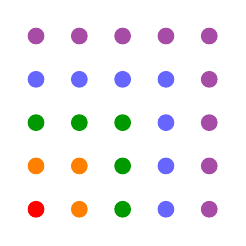
\begin{tikzpicture}[scale=0.55]

  % Colors for each gnomon
  % Gnomon 1: just (1,1) - 1 dot
  % Gnomon 2: 3 dots
  % Gnomon 3: 5 dots
  % Gnomon 4: 7 dots
  % Gnomon 5: 9 dots

  \def\dotradius{0.18}

  % Gnomon 5 (outermost) - purple - 9 dots
  % bottom row: (1,5)(2,5)(3,5)(4,5)(5,5)
  % right col: (5,1)(5,2)(5,3)(5,4)
  \foreach \x in {1,2,3,4,5} {
    \filldraw[violet!70] (\x, 5) circle (\dotradius);
  }
  \foreach \y in {1,2,3,4} {
    \filldraw[violet!70] (5, \y) circle (\dotradius);
  }

  % Gnomon 4 - blue - 7 dots
  \foreach \x in {1,2,3,4} {
    \filldraw[blue!60] (\x, 4) circle (\dotradius);
  }
  \foreach \y in {1,2,3} {
    \filldraw[blue!60] (4, \y) circle (\dotradius);
  }

  % Gnomon 3 - green - 5 dots
  \foreach \x in {1,2,3} {
    \filldraw[green!60!black] (\x, 3) circle (\dotradius);
  }
  \foreach \y in {1,2} {
    \filldraw[green!60!black] (3, \y) circle (\dotradius);
  }

  \foreach \x in {1,2} {
    \filldraw[orange] (\x, 2) circle (\dotradius);
  }
  \filldraw[orange] (2, 1) circle (\dotradius);

  \filldraw[red] (1, 1) circle (\dotradius);

\end{tikzpicture}
\end{center}

This is once again, another moment in which a diagram is expressly useful in a proof. The squares are organized by color. $1$ just leaves us with $1^2 = 1$. But now, when we add 3, which are the orange 3 dots, the total is now a $ 2 \times 2$ square. Next, consider the green dots. There are 5 green dots, and when we add it, we get a $3 \times 3$ square. This pattern continues with adding 7 blue dots, giving us a $4 \times 4$ square, and so on. This grid pattern shows us that as we add an odd number in an upside-down L shape, the square grows larger. But there is still one nagging question. How do we prove that each L shape is always an odd number of dots? Thankfully, the answer is quite simple. Consider a $k \times k$ square. To make it larger, we need to add $2k+1$ dots, which is the L-shape. We can see this visually in the grid, since we need to add $k$ dots on either side above and to the right of the original square, and add one more to fill in the missing gap in the top right corner. We can see that mathematically and visually, adding the $2k+1$ dots to a $k \times k$ square produces yet another. Consider the below diagram.

\begin{center}
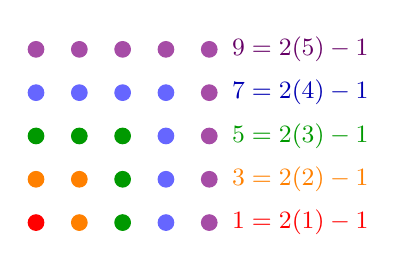
\begin{tikzpicture}[scale=0.55]

  \def\dotradius{0.18}

  \foreach \x in {1,2,3,4,5} {
    \filldraw[violet!70] (\x, 5) circle (\dotradius);
  }
  \foreach \y in {1,2,3,4} {
    \filldraw[violet!70] (5, \y) circle (\dotradius);
  }

  \foreach \x in {1,2,3,4} {
    \filldraw[blue!60] (\x, 4) circle (\dotradius);
  }
  \foreach \y in {1,2,3} {
    \filldraw[blue!60] (4, \y) circle (\dotradius);
  }

  \foreach \x in {1,2,3} {
    \filldraw[green!60!black] (\x, 3) circle (\dotradius);
  }
  \foreach \y in {1,2} {
    \filldraw[green!60!black] (3, \y) circle (\dotradius);
  }

  \foreach \x in {1,2} {
    \filldraw[orange] (\x, 2) circle (\dotradius);
  }
  \filldraw[orange] (2, 1) circle (\dotradius);

  \filldraw[red] (1, 1) circle (\dotradius);

  \node[violet!80!black, right] at (5.3, 5) {\small $9 = 2(5)-1$};
  \node[blue!70!black, right] at (5.3, 4) {\small $7 = 2(4)-1$};
  \node[green!60!black, right] at (5.3, 3) {\small $5 = 2(3)-1$};
  \node[orange, right] at (5.3, 2) {\small $3 = 2(2)-1$};
  \node[red, right] at (5.3, 1) {\small $1 = 2(1)-1$};

\end{tikzpicture}
\end{center}
This shows visually that adding $2k+1$ produces a larger square, and mathematically this is seen through the identity
\[
k^2 + (2k+1) = k^2 + 2k + 1 = (k+1)^2
\]
As we iterate $k$ from 1 and upward, we slowly grow the square, adding odd numbers after odd numbers, each of which increases the side length of the square by exactly one. This is why! As we increment the number of odd numbers, the square gets bigger. 
\end{proof}

Once again, we would not have been able to show that this identity holds for all odd numbers unless we had reasoned through the generic form of the pattern. Otherwise, we would be stuck brute forcing! Note again that our argument here was perhaps a bit informal, especially with the final identity and the iteration logic. We will fully formalize this in Volume 2, when we discuss inductive proofs. Our proof here started quite similar, we started with a base case (1), and showed that adding the next odd number increases the side length of the square by one, which is very close to becoming a full inductive proof. 

Yet again, this demonstrates both the importance of proofs and a beautiful way of actually doing a proof. Hopefully this has provided a little more motivation for you to study proofs!

\section{Problems}
\begin{problem}
With respect to the first example, try to wrap your head around why we are allowed to construct whatever figure we like. Convince yourself that this really does prove the Pythagorean Theorem for all right triangles. 
\end{problem}

\begin{problem}
I have used some symbols that you may not know the meanings for (yet). Look through the proofs, and see how many you can find. Can you infer the meanings? (Note that $\alpha, \beta, \gamma$ are Greek letters used as variable names and are not mathematical symbols in their own right). 
\end{problem}

\begin{problem}
Given that the center figure is just a rotated square, try to prove (or write the argument we used) the Pythagorean Theorem. 
\begin{center}
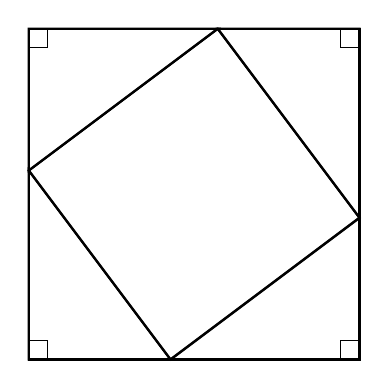
\begin{tikzpicture}[scale=0.6]

  % Outer square
  \draw[thick] (0,0) rectangle (7,7);

  % Inner tilted square
  \draw[thick] (3,0) -- (7,3) -- (4,7) -- (0,4) -- cycle;

  % Triangle outlines
  \draw[thick] (0,0) -- (3,0) -- (0,4) -- cycle;
  \draw[thick] (3,0) -- (7,0) -- (7,3) -- cycle;
  \draw[thick] (7,3) -- (7,7) -- (4,7) -- cycle;
  \draw[thick] (0,4) -- (0,7) -- (4,7) -- cycle;

  % Right angle boxes at OUTER corners
  \draw (0.4,0) -- (0.4,0.4) -- (0,0.4);
  \draw (6.6,0) -- (6.6,0.4) -- (7,0.4);
  \draw (7,6.6) -- (6.6,6.6) -- (6.6,7);
  \draw (0.4,7) -- (0.4,6.6) -- (0,6.6);
\end{tikzpicture}
\end{center}
\end{problem}

\begin{problem}
Using a similar geometric argument to the one in this chapter, find a visual 
"proof" (argument) that 
\[
\sum_{i=1}^{n} i = \frac{n(n+1)}{2}
\]
\hints{H26} \hfill $\star$
\end{problem}

\begin{problem}
    Consider the following pattern:
    \[
    1  = 1^3 = 1^2 = 1
    \]
    \[
    1 + 8 = 1^3 + 2^3 = 3^2 = 9
    \]
    \[
    1 + 8 + 27  = 1^3 + 2^3 + 3^3 = 6^2 = 36
    \]
    \[
    1 + 8 + 27 + 64 = 1^3 + 2^3 + 3^3 + 4^3 = 10^2 = 100
    \]
    What do you notice? Can you formulate a conjecture about the sum of the first $n$ perfect cubes? Test your conjecture for a few more values. Try to use summation notation to write down the formal, general, pattern.
\end{problem}